\documentclass[pt12]{beamer}
%\documentclass[pt12,externalviewer]{beamer}

\usepackage{verbatim}
\usepackage{amssymb}
\usepackage{graphicx}
%\usepackage{rotating}
%\usepackage{amsmath}
%\usepackage{tikz}
%\usepackage{beamergraphics}
\usepackage[]{babel}
%\usepackage[latin1]{inputenc}
\usepackage[T1]{fontenc}
\newcommand{\av}[1]{\langle #1 \rangle}
\newcommand{\mel}[3]{\langle#1|#2|#3\rangle}
\newcommand{\ket}[1]{|#1\rangle}
\newcommand{\scal}[2]{\langle #1|#2\rangle}
\newcommand{\ord}[1]{^{(#1)}}
\newcommand{\bra}[1]{\langle #1|}
\newcommand{\limit}[2]{\lim_{#1 \to #2}}

%\usepackage[absolute,overlay]{textpos}
%\usepackage{pdfcolparallel}

%\usepackage{tcolorbox}
%\tcbuselibrary{fitting}

\definecolor{CTgreen}{HTML}{28794e} % Catania green (primary)
\definecolor{UBCblue}{rgb}{0.02706, 0.04725, 0.526667} % UBC Blue (primary)
%\definecolor{UBCblue}{rgb}{0.01706, 0.03725, 0.426667} % UBC Blue (primary)
\mode<presentation>
{
  \usetheme{Warsaw}
%  \usetheme{Madrid}
%  \usetheme{Montpellier}
%  \usetheme{Marburg}
  \usecolortheme[named=UBCblue]{structure}
  \setbeamercolor{alerted text}{fg=blue}
  \setbeamercovered{transparent}
  \setbeamertemplate{section in toc}[ball unnumbered]
}

%\setbeamertemplate{footline}{\hfill\insertframenumber/\inserttotalframenumber}

\expandafter\def\expandafter\insertshorttitle\expandafter{%
  \insertshorttitle\hfill%
  \insertframenumber\,/\,\inserttotalframenumber}

\newcommand{\backupbegin}{
   \newcounter{framenumberappendix}
   \setcounter{framenumberappendix}{\value{framenumber}}
}
\newcommand{\backupend}{
   \addtocounter{framenumberappendix}{-\value{framenumber}}
   \addtocounter{framenumber}{\value{framenumberappendix}}
}

\newcommand{\refer}[1]{%
   \begin{flushright}
      {\alert{\tiny #1}}
   \end{flushright}}

\newcommand{\lrefer}[1]{%
   \begin{flushleft}
      {\alert{\tiny #1}}
   \end{flushleft}}

\newcommand{\param}[1]{%
   \begin{flushright}
      {\small #1}
   \end{flushright}
   \vspace{-1.5\baselineskip}
}

\newcommand{\sech}{\mathop{\rm sech}\nolimits}
\newcommand{\sgn}{\mathop{\rm sgn}\nolimits}
\newcommand{\etal}{{\em et al.}}


\title{The Quark-Photon Vertex BSE}

\author{S. Hagel, L. Kiefer, F. Murgana, F.R. Sattler, J. Wessely}



\date{18. May 2022}

\begin{document}

\begin{frame}[plain]
\titlepage
\end{frame}



\begin{frame}[label=outline]
\frametitle{Outline}
\tableofcontents[pausesections]
\end{frame}

\section{Motivation}
 \begin{frame}\frametitle{Motivations}



\begin{itemize}
	\item Electromagnetic form factor;
	\item Anomalous magnetic moment;
\end{itemize}
\vspace{2mm}

The coupling of a photon to an onshell spin-$1/2$ fermion with mass $m$ is described by the electromagnetic
current matrix element
\begin{equation}
	J^\mu(k, Q)=i\bar{u}(k_+)\left[F_1(Q^2)\gamma^\mu-\frac{F_2(Q^2)}{2m}\sigma^{\mu\nu}Q^\nu\right]u(k_-)
\end{equation}

Quarks are not onshell \\
\hspace{2cm}$\Rightarrow$ $3$ Lorentz invariants ($Q^2, k^2, Q\cdot k$)\\
\vspace{2mm}
\hspace{2cm}$\Rightarrow$ $12$ Lorentz-Dirac tensors.\\
\vspace{2mm}
\hspace{2cm}$\Rightarrow$ $12$ dressing functions $F_i(k^2, k\cdot Q, Q^2)$

\end{frame}

\endinput


\section{The Quark-Photon Vertex BSE}

\begin{frame}\frametitle{Quark-Photon Vertex}
\begin{minipage}[r]{0.49\textwidth}
	\hspace{2mm}
	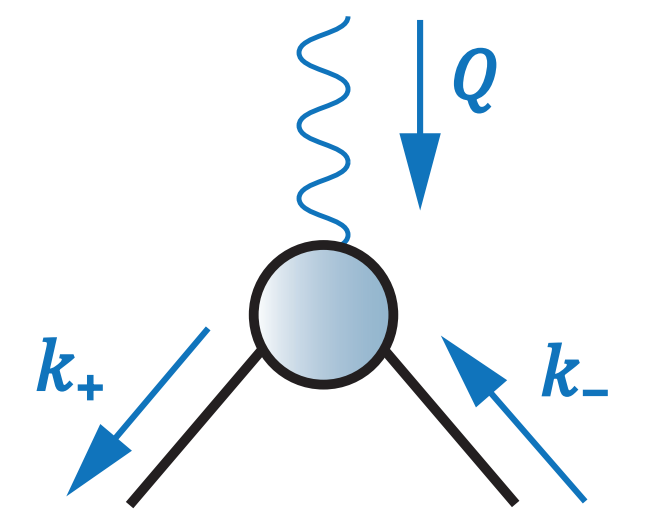
\includegraphics[height=2.2cm, width=3.2cm]{Vertex.png}
\end{minipage}
%
\begin{minipage}[r]{0.49\textwidth}
\begin{align}
k_{\pm} =& k \pm \frac{Q}{2} \\\nonumber
k_{\pm}^2=& k² \pm \frac{Q^2}{4} \pm Q\cdot k
\end{align}
\end{minipage}\\
%
\vspace{3mm}
%

In general, quarks are not on-shell \\
\hspace{2cm}$\Rightarrow$ $3$ Lorentz invariants ($Q^2, k^2, Q\cdot k$)\\
\vspace{2mm}
\hspace{2cm}$\Rightarrow$ $12$ Lorentz-Dirac tensors.\\
\vspace{2mm}
\hspace{2cm}$\Rightarrow$ $12$ dressing functions $F_i(k^2, k\cdot Q, Q^2)$
\end{frame}

\begin{frame}\frametitle{Quark-Photon Vertex}
The quark-photon vertex must satisfy electromagnetic gauge invariance in the form of the
Ward-Takahashi identity (WTI):

\begin{equation}
	Q^\mu\Gamma^\mu(k, Q)=S(k_+)^{-1}-S(k_-)^{-1}
\end{equation}

\begin{minipage}[r]{0.65\textwidth}
	$\rightarrow$ Split vertex in transverse and longitudinal parts $T_i^{\mu} \; \text{and} \; G_j^{\mu} $ with respect to incoming photon momentum:
\end{minipage}
\begin{minipage}[r]{0.30\textwidth}
	\hspace{2mm}
	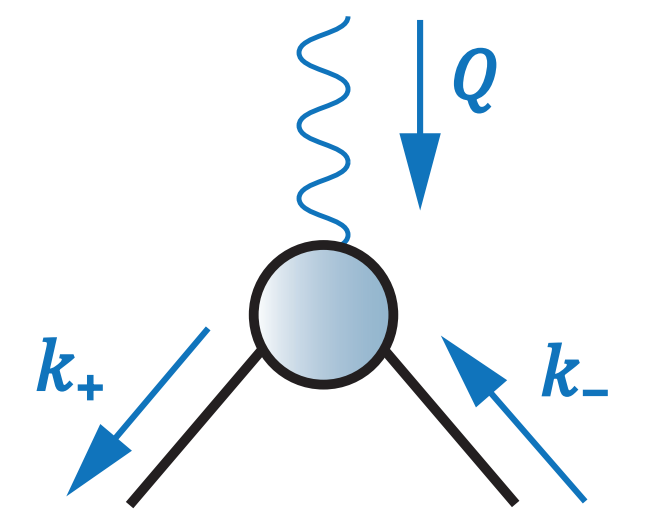
\includegraphics[height=2.2cm, width=3.2cm]{Vertex.png}
\end{minipage}

\begin{equation}
	\Gamma^\mu(k,Q)=\sum_{j=1}^4 g_j(k^2, \omega, Q^2)iG^\mu_j(k, Q)+\sum_{j=1}^8 f_j(k^2, \omega, Q^2)iT^\mu_j(k, Q)
\end{equation}

\end{frame}



\begin{frame}\frametitle{Quark-Photon Vertex}
With this decomposition,[[should we show this slide???] the vertex has a charge-conjugation symmetry

\begin{equation}
	\bar{\Gamma}^\mu(k,Q):=-C\Gamma^\mu(-k,Q)^TC^T=\Gamma^\mu(k, -Q) \qquad C=\gamma^4\gamma^2
\end{equation}
\vspace{4mm}
It is easy to show that each $G_j^\mu$, $T_j^\mu$
satisfies the same relation $\Rightarrow$\\ \vspace{3mm} $g_j(k^2, \omega, Q^2)=g_j(k^2, \omega^2, Q^2)$, $\qquad$ $f_j(k^2, \omega, Q^2)=f_j(k^2, \omega^2, Q^2)$\\

\vspace{9mm}

The tensor basis  is free of kinematic constraints $\Rightarrow$
\vspace{2mm}
$g_j(k^2, \omega^2,Q^2)$ and $f_j(k^2, \omega^2,Q^2)$ become constant for $Q^\mu\to0$ or $k_\mu\to  0$.

\end{frame}


\endinput


\section{Bethe-Salpeter equation (BSE)}
\begin{frame}\frametitle{Bethe-Salpeter equation}
To calculate the quark-photon vertex dynamically, we can solve its Bethe-Salpeter equation:
\begin{figure}[h]
	\centering
	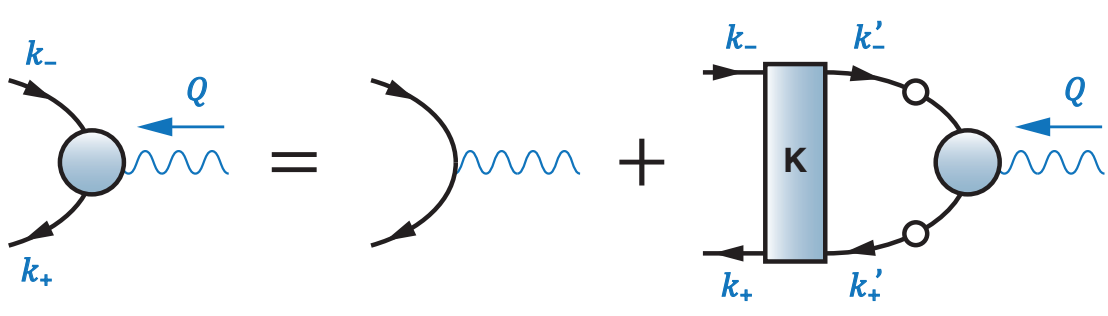
\includegraphics[height=2.7cm, width=10.2cm]{BSE.png}
\end{figure}
\textit{Rainbow-ladder truncation}: approximate the full kernel by
a gluon exchange with an effective interaction given by the Maris-Tandy model


\end{frame}

\begin{frame}\frametitle{Bethe-Salpeter equation}

\begin{equation}
	g(k^2)=Z^2_2\frac{16\pi}{3}\frac{\alpha(k^2)}{k^2}
\end{equation}

\begin{equation}
\alpha(k^2)=\pi \eta^7 x^2 e^{-\eta^2 x} + \frac{2\pi\gamma_m\left(1-e^{k^2/\Lambda_t^2}\right)}{\ln\left[e^2 - 1 + \left(1 + \frac{k^2}{\Lambda_{QCD}^2}\right)^2\right]}, \qquad x=\frac{k^2}{\Lambda^2}
\end{equation}

The resulting BSE reads explicitly:
\begin{equation}
	\Gamma^\mu(k, Q)=Z_2i\gamma^\mu+\int_{k'}\!\!g(l^2)T^{\alpha\,\beta}_l\gamma^\alpha S(k'_+)\Gamma^\mu(k', Q)S(k'_-)\gamma^\beta
\end{equation}
\end{frame}

\endinput

\section{Pulsar Glitches and Superfluidity}

%
\begin{frame}\frametitle{Solving the BSE}

We rewrite the decomposition as
\small\begin{equation}
\!\!\!\!\!\!\!	\Gamma^\mu(k, Q)=\sum_{j=1}^{12} F_j(k^2, \omega, Q^2)it^\mu_j(k,Q), \quad F_j\in\{g_j,f_j\}, \; t^\mu\in\{G^\mu_j, T^\mu_j\}
\end{equation}

$$\!\!\!\!\!\!\!\!\!H_{ij}(k^2, \omega, Q^2)=1/4\mbox{Tr}\left\{\bar{t}^\mu_i(k,Q)t^\mu_j(k,Q)\right\}\neq\delta_{ij}\Longrightarrow t^\mu_j  \mbox{ not ortonormal }$$
We want to construc an orthonormal basis $H_{ij}=\delta_{ij}$
Fisrt we choose a frame for the four vectors:
\begin{figure}[!htb]

	\minipage{0.32\textwidth}
	\hspace{-7mm}
	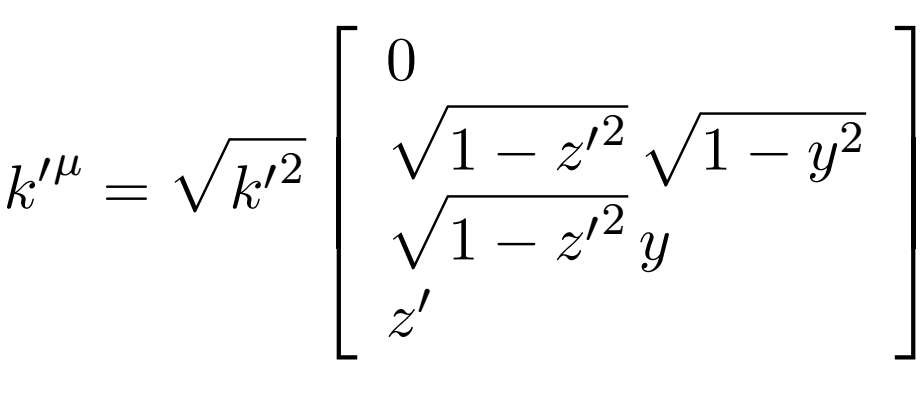
\includegraphics[width=4cm, height=2cm]{kps.png}

	\endminipage\hfill
	\minipage{0.32\textwidth}
	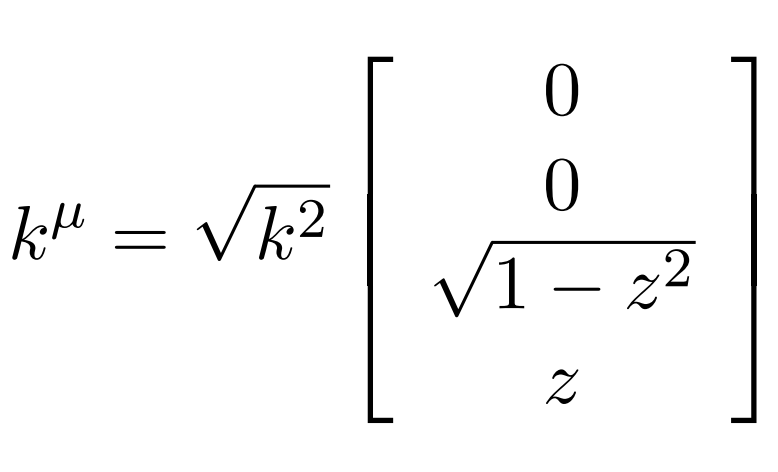
\includegraphics[width=\linewidth]{ks.png}

	\endminipage\hfill
	\minipage{0.32\textwidth}%
	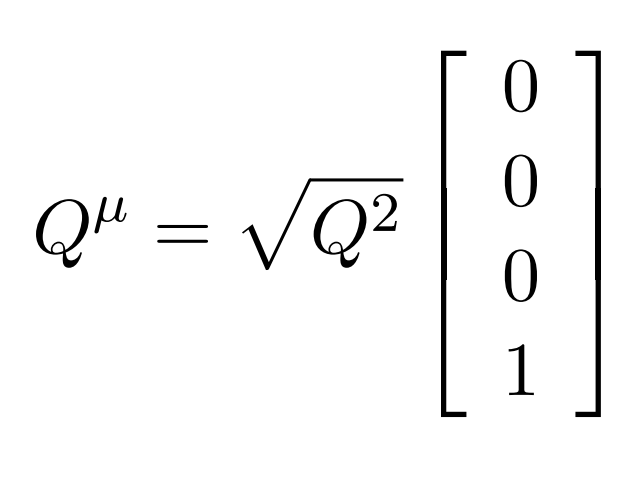
\includegraphics[width=\linewidth,  height=2.3cm]{Qs.png}

	\endminipage
\end{figure}



\end{frame}

\begin{frame}
	In this way we can express the quark-photon vertex in the following basis:
	\begin{equation}
		\Gamma^\mu(k, Q)=\sum_{j=1}^{12}a_(k^2, \omega, Q^2)i\tau_j^\mu(k,Q)
	\end{equation}
with
\begin{figure}
		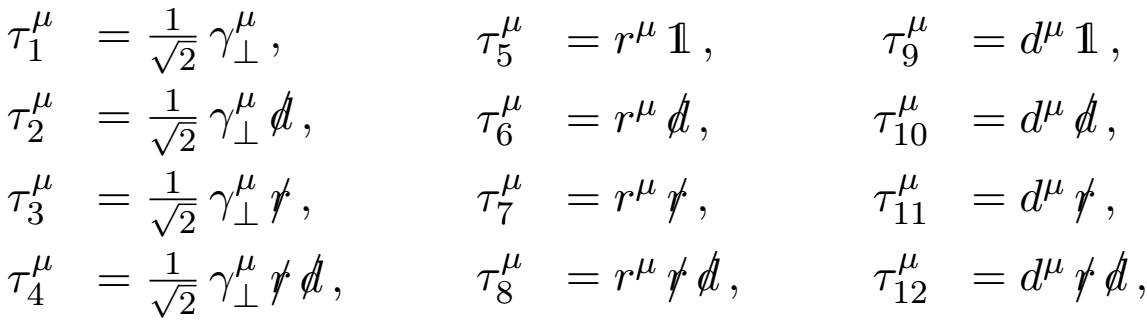
\includegraphics[width=\linewidth,  height=2.3cm]{taus.png}
\end{figure}
\end{frame}

\endinput


\section{Starquakes}
%\include{slide5}

%\include{conclusions}

%\appendix
%\backupbegin

%\section*{Parte ausiliaria}
%\include{slideaux1}




\end{document}

